\subsection{Motivation}

\begin{frame}
\frametitle{Motivation}
  \begin{itemize}
    \item 
  \end{itemize}
\end{frame}


\subsection{Objectives}

\begin{frame}
\frametitle{Objectives}
  \begin{itemize}
    \item 
  \end{itemize}
\end{frame}


\subsection{MOOSE}

\begin{frame}
\frametitle{MOOSE}
\begin{columns}
    \column[t]{4cm}
	\begin{itemize}
    	\item Computational framework
    	\item Solves coupled equation systems
    	\item MOOSE defines weak forms
    	\item MOOSE and LibMesh translate them into residual and Jacobian functions
    	\item PetSc solution routines solve the equations
    \end{itemize}

	\column[t]{6cm}
	\begin{figure}[htbp!]
		\begin{center}
			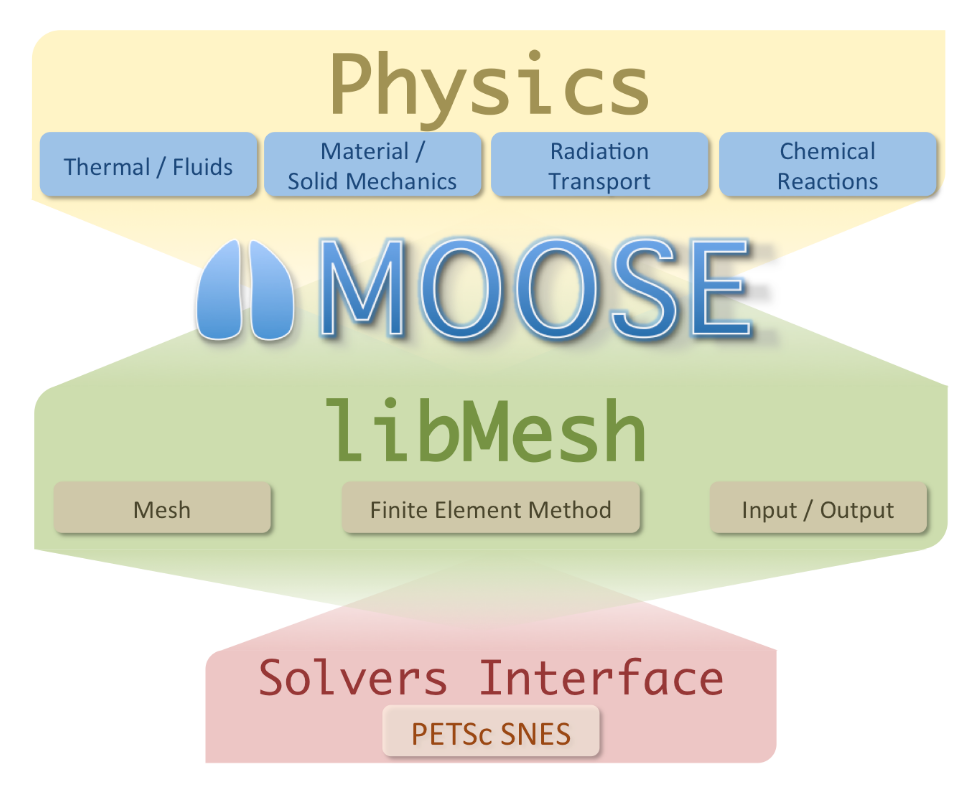
\includegraphics[width=6cm]{figures/moose}
		\end{center}
		\caption{MOOSE framework. Image reproduced from \cite{inl_workshop_2020}.}
	\end{figure}
\end{columns}
\end{frame}
